\begin{frame}{7.1 Arsitektur Sirkuit QPCA 4x4}
    \begin{columns}
        \begin{column}{0.6\textwidth}
            \centering
            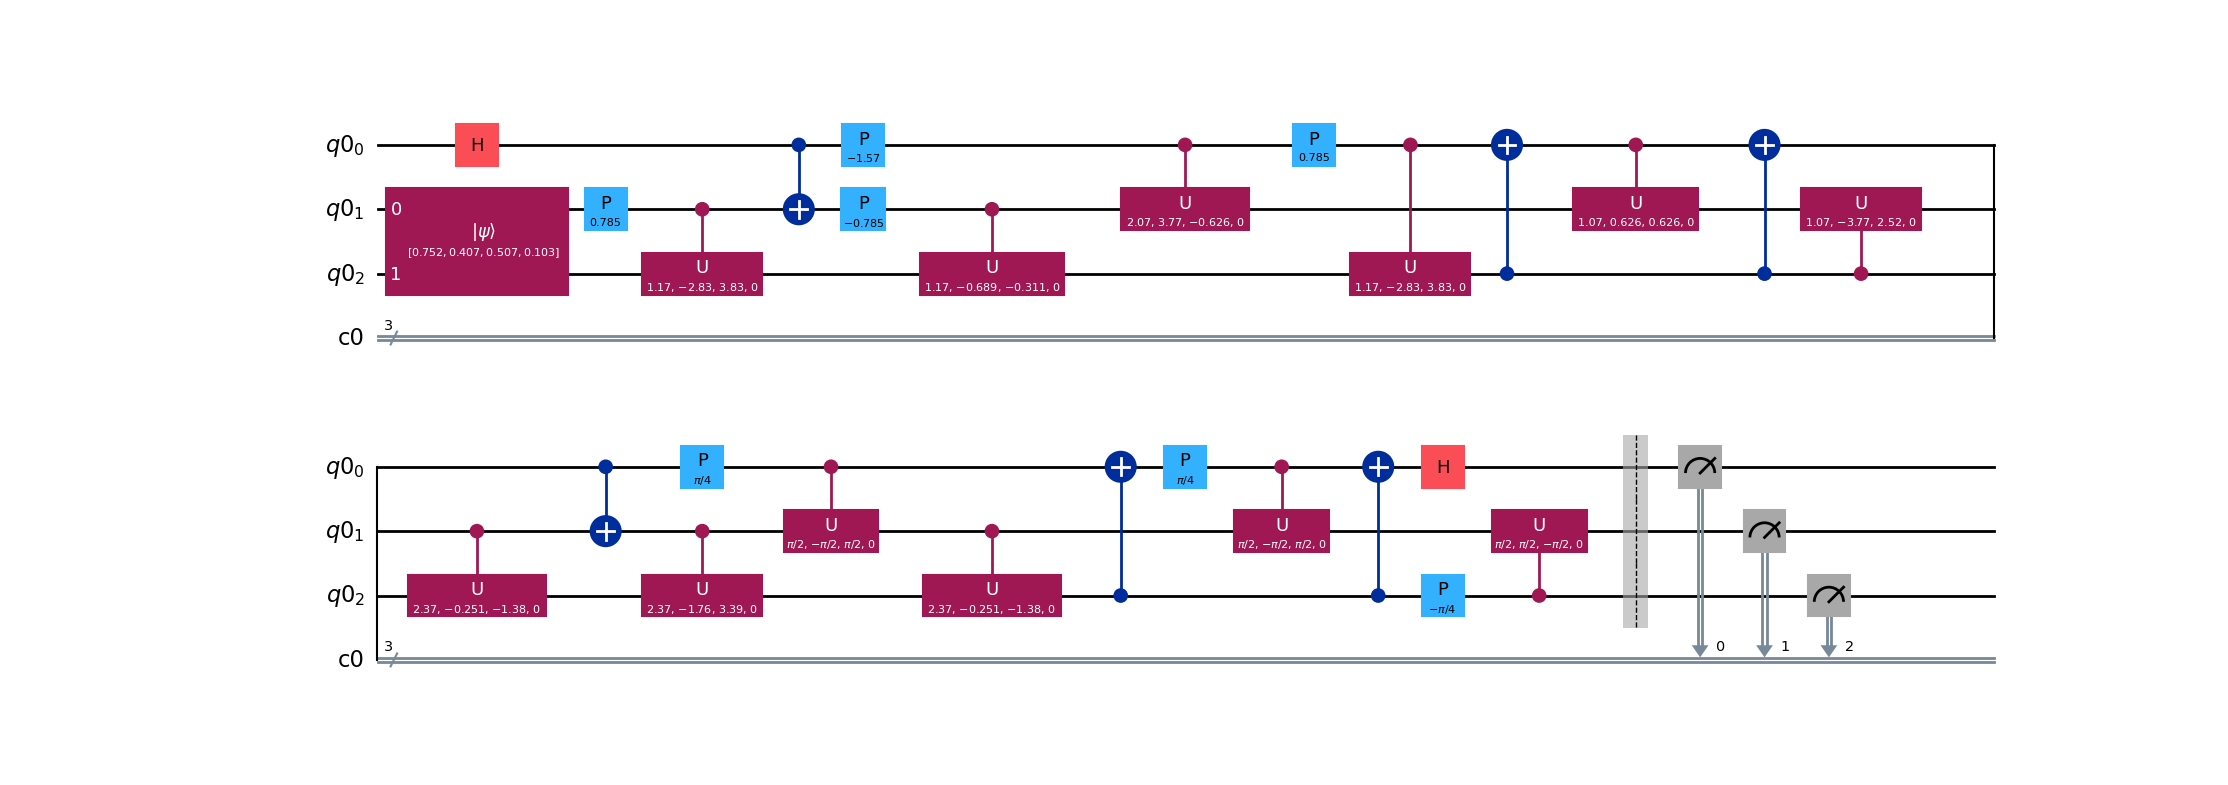
\includegraphics[width=\textwidth]{../QPCA-master/circuit_4x4.png}
            \captionof{figure}{Sirkuit QPCA Multivariat}
        \end{column}
        \begin{column}{0.4\textwidth}
            \small
            \begin{itemize}
                \item \textbf{Register Target ($q_1, q_2$):} Menyandikan korelasi silang antara tiga tenor maturitas (4-state basis).
                \item \textbf{Kedalaman Sirkuit:} Terdiri dari 28 operasi gerbang yang disusun secara sekuensial.
                \item \textbf{Tantangan NISQ:} Struktur sirkuit yang panjang meningkatkan risiko dekoherensi fasa.
            \end{itemize}
        \end{column}
    \end{columns}
\end{frame}

\begin{frame}{7.2 Dekomposisi Sirkuit: Transpiled 4x4}
    \begin{columns}[t]
        \begin{column}{0.6\textwidth}
            \centering
            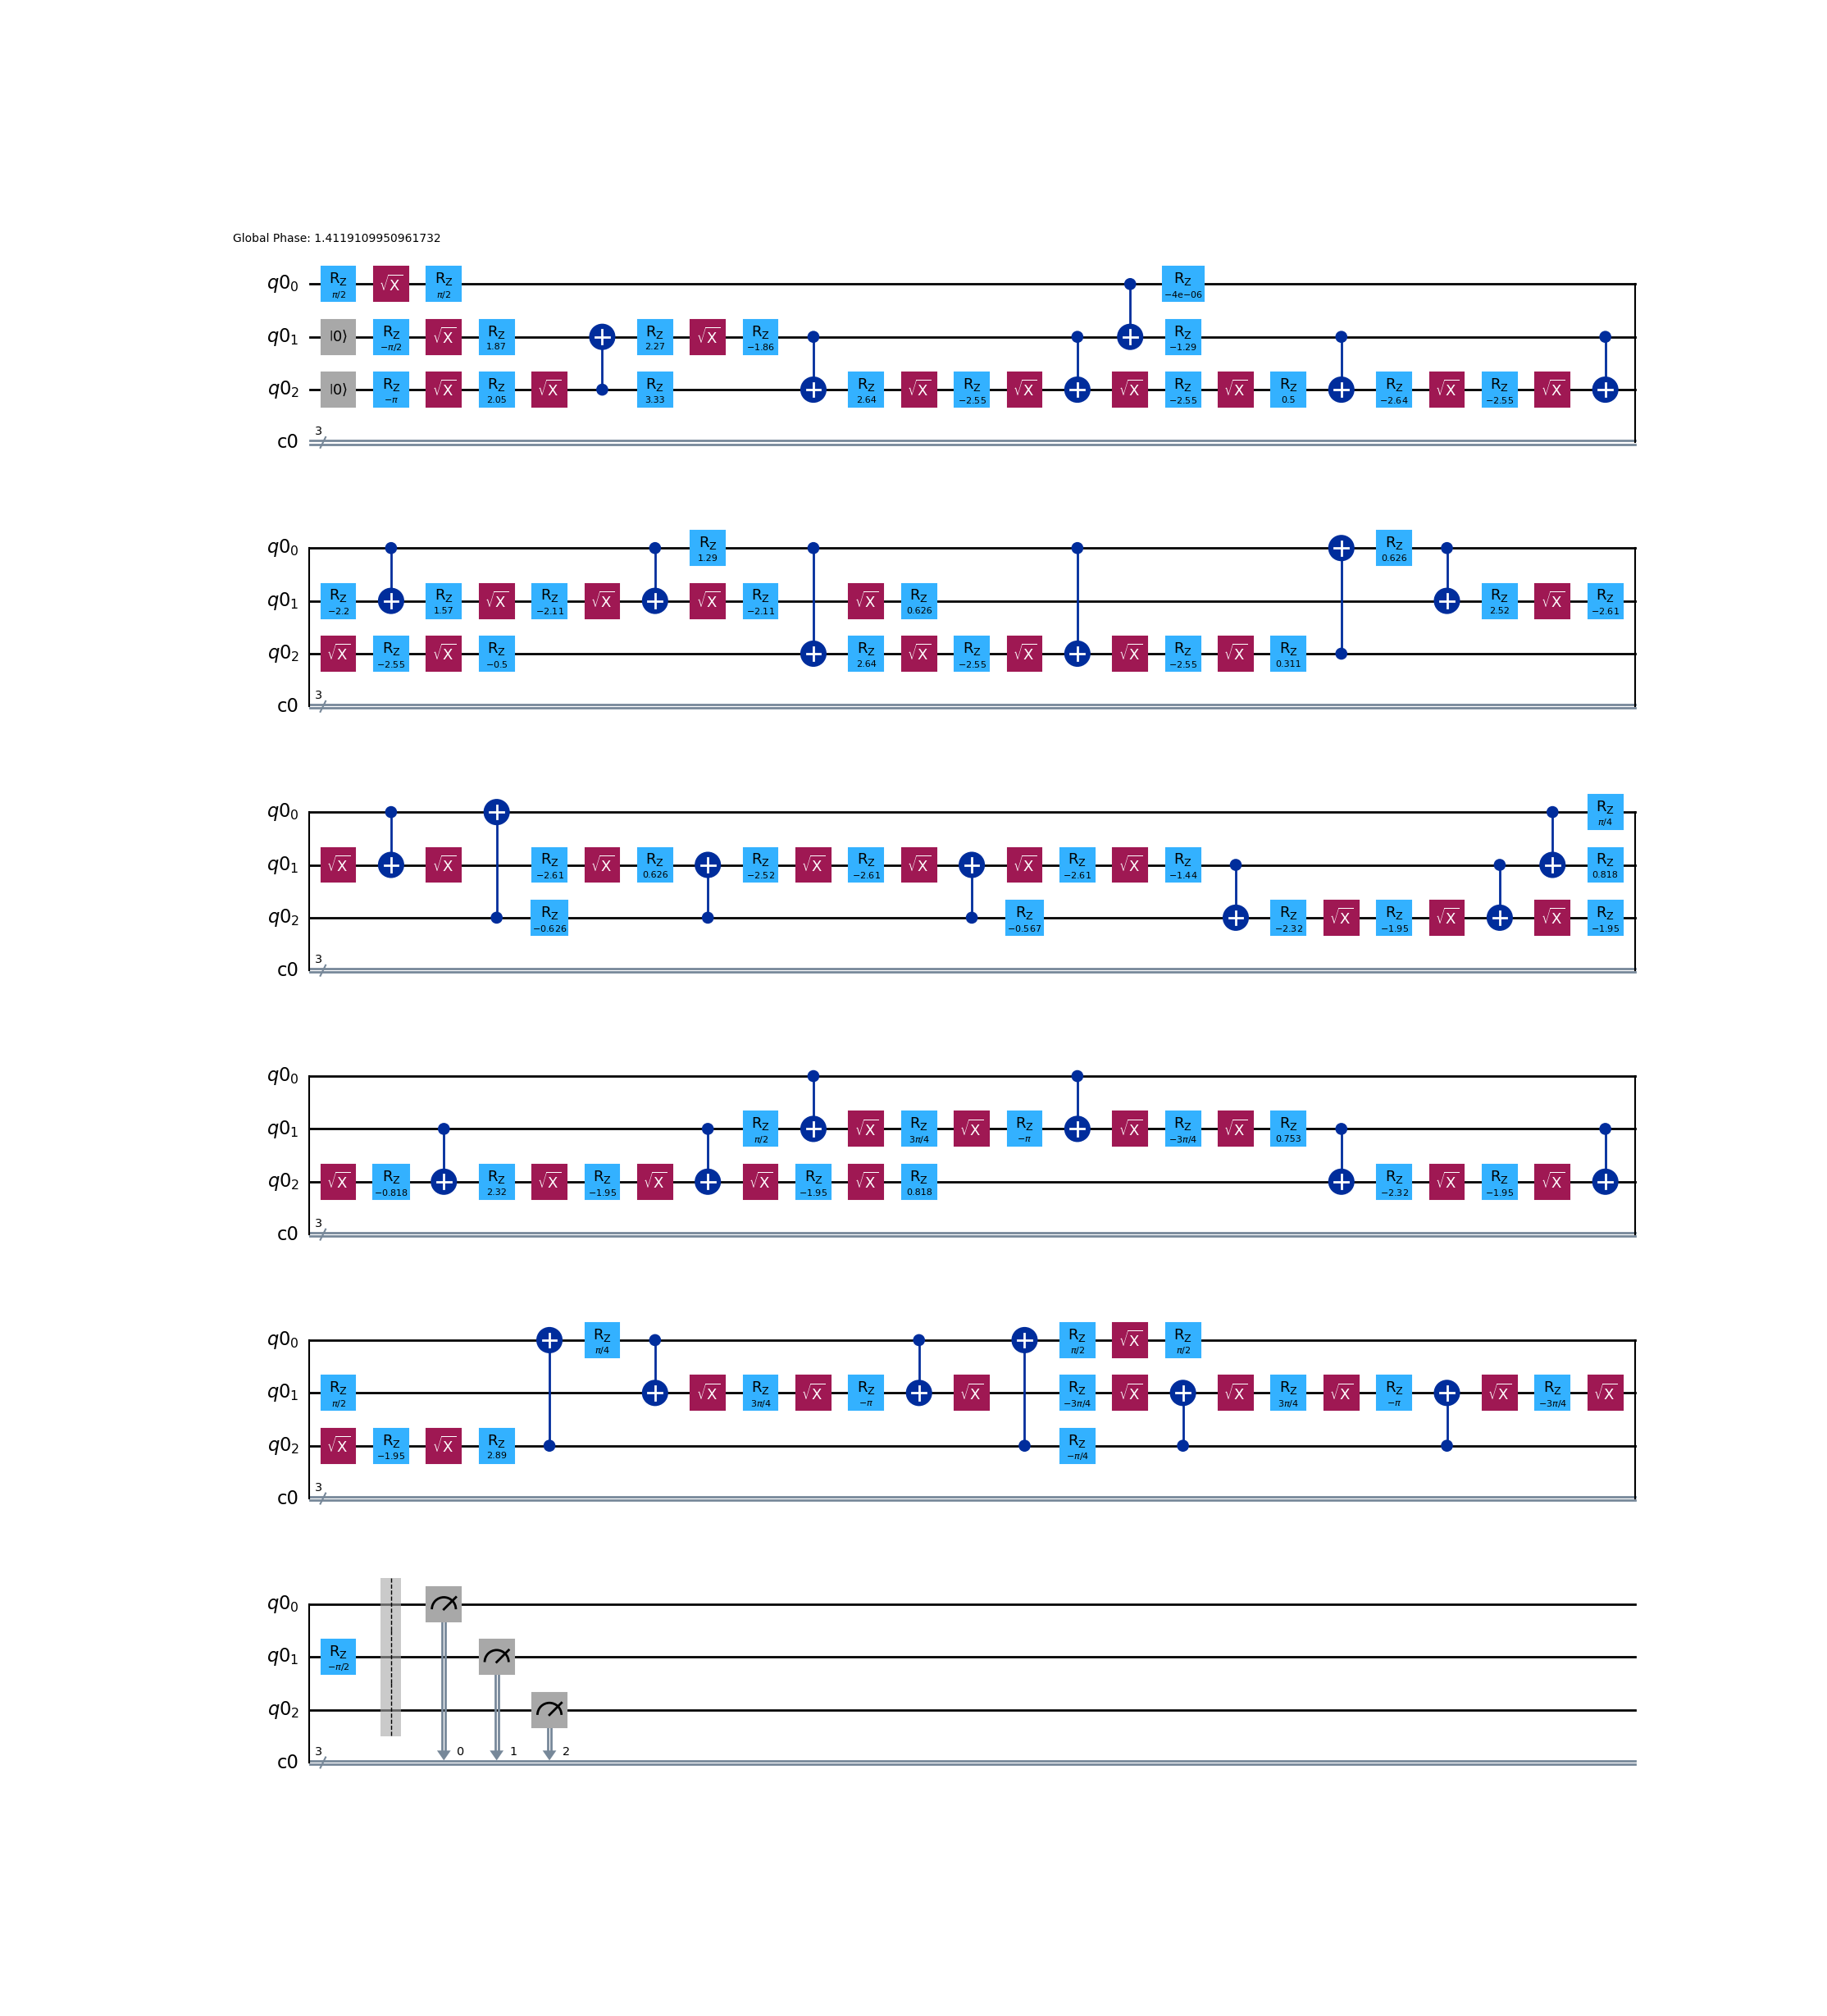
\includegraphics[width=0.75\textwidth]{../QPCA-master/circuit_transpiled_4x4.png}
            \captionof{figure}{Sirkuit 4x4 setelah Transpilasi}
        \end{column}
        \begin{column}{0.4\textwidth}
            \vspace*{-6cm}
            \small
            \begin{itemize}
                \item \textbf{Akumulasi Gerbang Fisik:} Transpilasi mengungkap lonjakan jumlah gerbang $CX$ untuk uniter $4 \times 4$.
                \item \textbf{Efek Komulatif Galat:} Setiap gerbang tambahan meningkatkan peluang galat fase dan relaksasi qubit.
                \item \textbf{Analisis Kedalaman:} Kedalaman sirkuit yang tinggi menjelaskan distribusi probabilitas yang menjadi uniform.
            \end{itemize}
        \end{column}
    \end{columns}
\end{frame}

\begin{frame}{7.3 Analisis Galat: Histogram Probabilitas 4x4}
    \begin{columns}
        \begin{column}{0.5\textwidth}
            \centering
            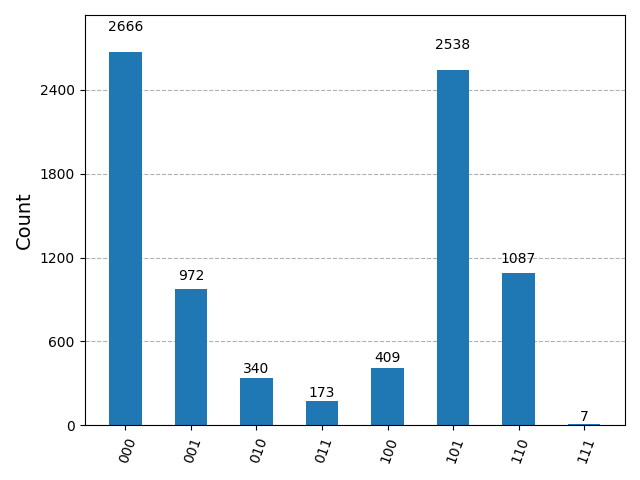
\includegraphics[width=\textwidth]{../QPCA-master/qpca_4x4_result.png}
            \captionof{figure}{Distribusi Probabilitas Terdegradasi}
        \end{column}
        \begin{column}{0.5\textwidth}
            \small
            \begin{itemize}
                \item \textbf{Distribusi Uniform:} Histogram menunjukkan probabilitas yang hampir merata. Informasi fase telah "terhapus" akibat akumulasi galat sirkuit.
                \item \textbf{Rasio Signal-to-Noise:} Dekoherensi sistemik menghambat ekstraksi \textit{eigenvalue} secara langsung tanpa teknik mitigasi.
            \end{itemize}
        \end{column}
    \end{columns}
\end{frame}

\begin{frame}{7.4 Tomografi 4x4: Analisis State City}
    \begin{columns}
        \begin{column}{0.5\textwidth}
            \centering
            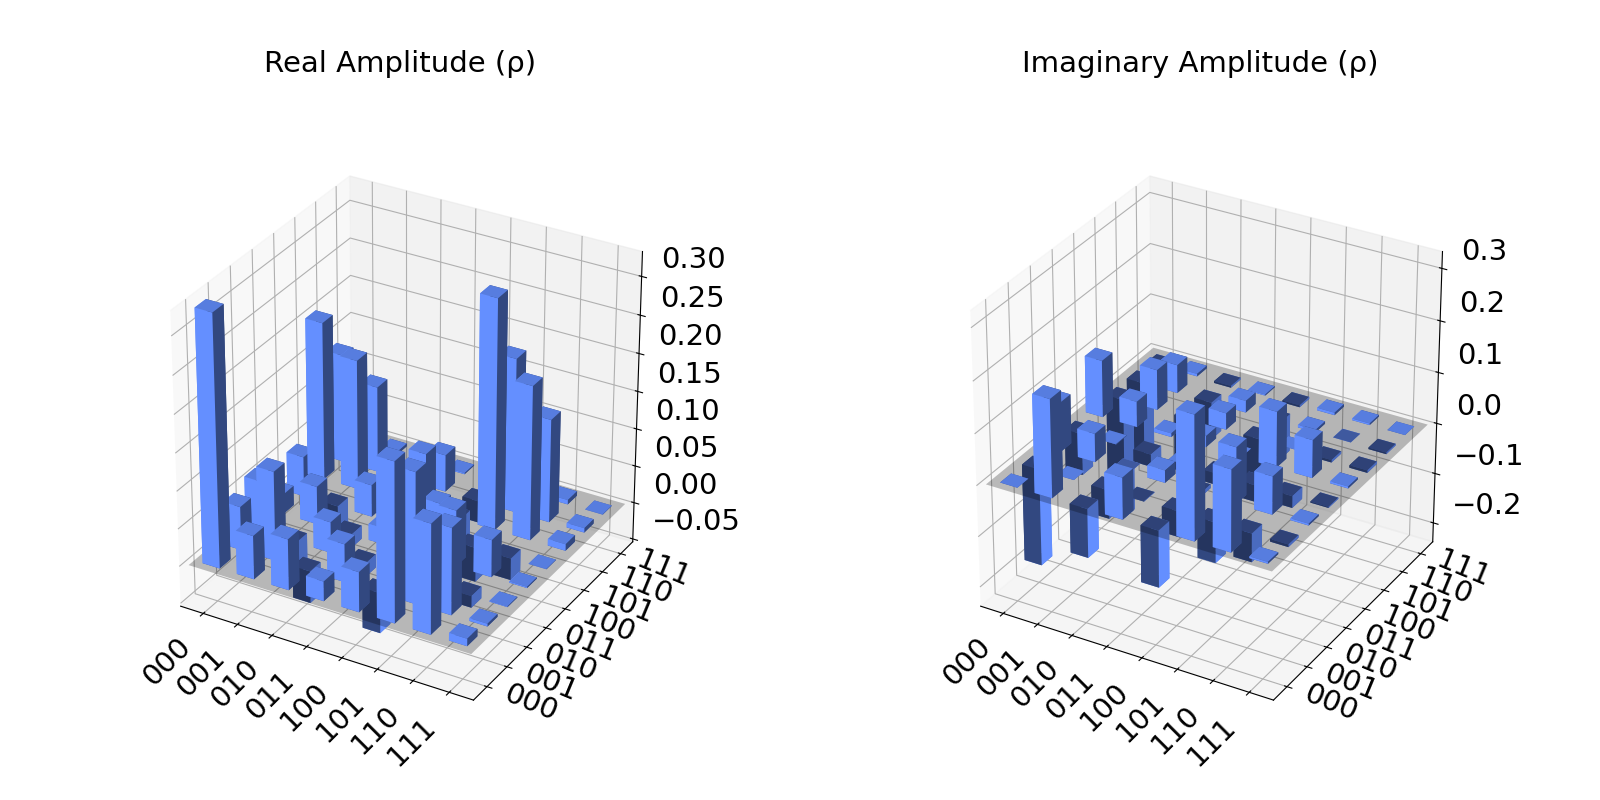
\includegraphics[width=\textwidth]{../QPCA-master/state_city_4x4.png}
            \captionof{figure}{Matriks Densitas 4x4 (Real)}
        \end{column}
        \begin{column}{0.5\textwidth}
            \small
            \begin{itemize}
                \item \textbf{Kebocoran Amplitudo:} Munculnya bar pada elemen-elemen matriks yang seharusnya nol merupakan bukti degradasi fidelitas \textit{state}.
                \item \textbf{Struktur Eigenvector:} Ketidakmampuan sistem mempertahankan puncak diagonal mencerminkan hilangnya integritas struktur \textit{eigenvector}.
            \end{itemize}
        \end{column}
    \end{columns}
\end{frame}

\begin{frame}{7.5 Degradasi Korelasi pada Hinton Map 4x4}
    \begin{columns}
        \begin{column}{0.5\textwidth}
            \centering
            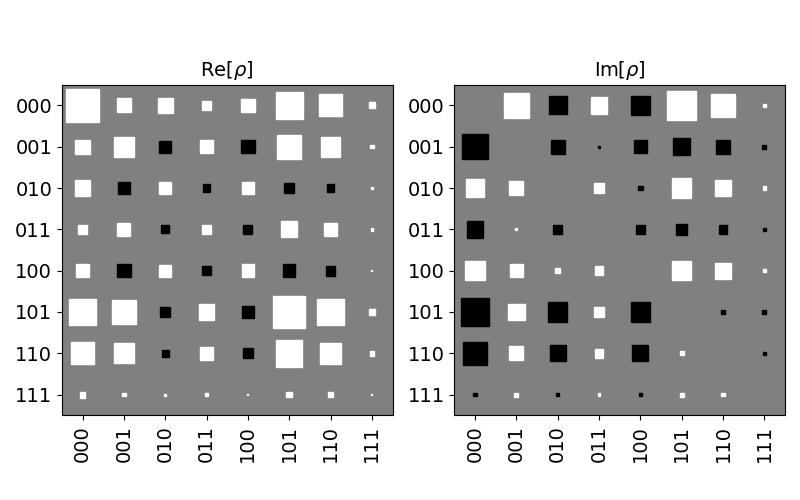
\includegraphics[width=0.9\textwidth]{../QPCA-master/hinton_4x4.png}
            \captionof{figure}{Hinton Map 4x4: Korelasi Kabur}
        \end{column}
        \begin{column}{0.5\textwidth}
            \small
            \begin{itemize}
                \item \textbf{Pola Koordinat:} Kotak-kotak putih terlihat mengecil dan tersebar, menunjukkan disrupsi hubungan \textit{entanglement} oleh noise.
                \item \textbf{Implikasi:} Peningkatan dimensi matriks memerlukan qubit dengan tingkat fidelitas gerbang dua-qubit yang jauh lebih tinggi.
            \end{itemize}
        \end{column}
    \end{columns}
\end{frame}

\begin{frame}{7.6 Kehilangan Koherensi pada Bola Bloch 4x4}
    \begin{columns}
        \begin{column}{0.5\textwidth}
            \centering
            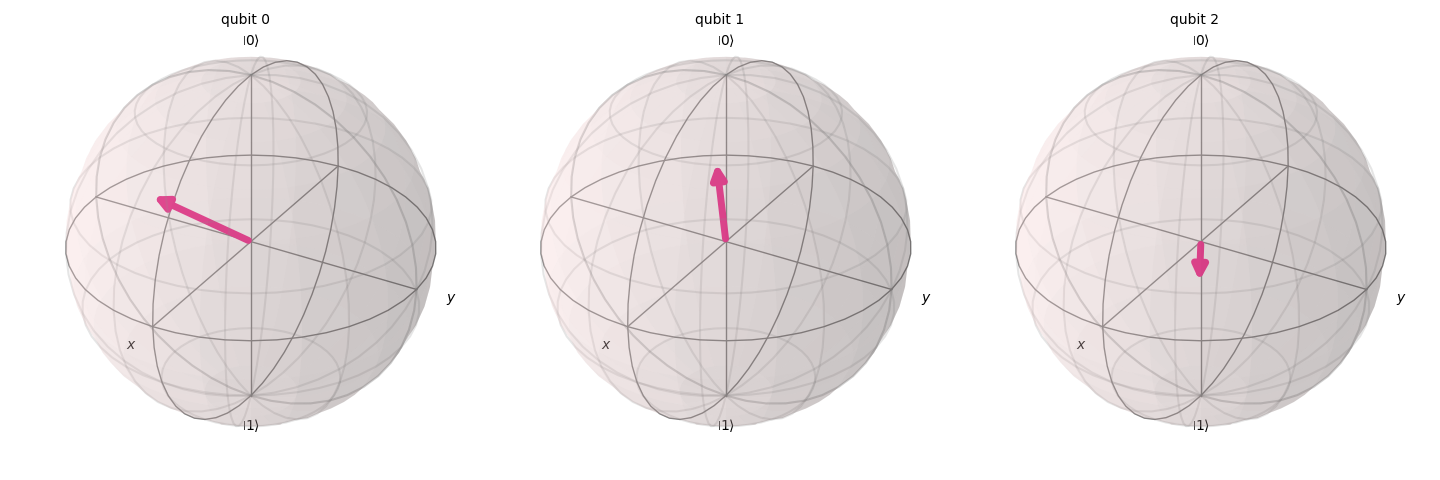
\includegraphics[width=\textwidth]{../QPCA-master/bloch_4x4.png}
            \captionof{figure}{Multivektor Bloch 4x4}
        \end{column}
        \begin{column}{0.5\textwidth}
            \small
            \begin{itemize}
                \item \textbf{Kontraksi Vektor:} Pemendekan panjang vektor ($r < 1$) mengindikasikan transisi dari \textit{pure state} menuju \textit{mixed state}.
                \item \textbf{Disorientasi Fase:} Akumulasi fase parasit merusak akurasi kalkulasi spektral finansial akibat noise sistemik.
            \end{itemize}
        \end{column}
    \end{columns}
\end{frame}
